%! Author = Adam
%! Date = 04/01/2026

\chapter{Prezentacja systemu}
\label{ch:prezentacja-systemu}

W niniejszym rozdziale przedstawiono finalny wygląd aplikacji.
Wcześniej opracowany projekt interfejsu zaprezentowany w rozdziale
\hyperref[sec:architektura-interfejsu-uzytkownika]{\ref*{sec:architektura-interfejsu-uzytkownika} Architektura interfejsu użytkownika}
pełnił funkcję punktu wyjścia oraz wsparcia w procesie implementacji.
Ostateczny kształt interfejsu został wypracowany iteracyjnie, na podstawie konsultacji
między członkami zespołu oraz z promotorem, a także wniosków wynikających z testów manualnych.
Z tego względu w wielu miejscach warstwa wizualna różni się od pierwotnych makiet.

\subimport{chapters/prezentacja-systemu/sections/}{strona-glowna.tex}
\subimport{chapters/prezentacja-systemu/sections/}{strona-mapy.tex}
\subimport{chapters/prezentacja-systemu/sections/}{strona-chatu.tex}
\subimport{chapters/prezentacja-systemu/sections/}{strona-forum.tex}
\subimport{chapters/prezentacja-systemu/sections/}{panel-logowania.tex}
%! Author = Mateusz
%! Date = 29/12/2025

\section{Panel użytkownika}
\label{sec:panel-uzytkownika}

Po zalogowaniu udostępniany jest panel użytkownika.
Nawigacja odbywa się z poziomu menu bocznego, a wybrane pozycje są wyróżniane (rys. \ref{fig:profile-main}).
Panel składa się z ośmiu sekcji:
\begin{itemize}
    \item Profile
    \item Spots
    \item Photos
    \item Movies
    \item Social
    \item Add spot
    \item Comments
    \item Settings
\end{itemize}


\subsubsection{Profile}

Domyślnym widokiem po wejściu do panelu jest profil użytkownika (rys. \ref{fig:profile-main}).
W górnej części prezentowane są podstawowe informacje oraz statystyki
(liczba znajomych, obserwowanych, obserwujących i dodanych zdjęć).
Poniżej wyświetlana jest sekcja najpopularniejszych zdjęć.

\begin{figure}[H]
    \centering
    \includegraphics[width=1\textwidth]{attachments/prezentacja-systemu/panel-uzytkownika/profile}
    \caption{Widok profilu użytkownika w panelu.}
    \label{fig:profile-main}
\end{figure}

Po najechaniu kursorem na zdjęcie profilowe pojawia się opcja zmiany zdjęcia (rys. \ref{fig:profile-change-photo}).
Rozwiązanie to umożliwia szybkie wykonanie akcji bez przechodzenia do osobnego formularza.

\begin{figure}[H]
    \centering
    \includegraphics[width=1\textwidth]{attachments/prezentacja-systemu/panel-uzytkownika/profile-change-photo}
    \caption{Akcja zmiany zdjęcia profilowego dostępna po najechaniu kursorem.}
    \label{fig:profile-change-photo}
\end{figure}

W sekcji najpopularniejszych zdjęć zastosowano efekt najechania (hover), który przyciemnia fragment ze statystykami
zdjęcia, poprawiając czytelność ikon i liczników (rys. \ref{fig:profile-photo-hover}).

\begin{figure}[H]
    \centering
    \includegraphics[width=1\textwidth]{attachments/prezentacja-systemu/panel-uzytkownika/profile-hover}
    \caption{Efekt najechania na kafelek zdjęcia (podkreślenie statystyk).}
    \label{fig:profile-photo-hover}
\end{figure}

Dostępny jest również motyw ciemny (rys. \ref{fig:profile-dark}).

\begin{figure}[H]
    \centering
    \includegraphics[width=1\textwidth]{attachments/prezentacja-systemu/panel-uzytkownika/profile-dark}
    \caption{Profil użytkownika w trybie ciemnym.}
    \label{fig:profile-dark}
\end{figure}

Profil może zostać wyświetlony również w trybie podglądu innego użytkownika (np. po wejściu z sekcji Social).
W takim przypadku prezentowane są dane danego profilu oraz dostępne są akcje społeczne
(obserwowanie/usunięcie ze znajomych) (rys. \ref{fig:profile-friend}).
Kliknięcie w wybrane statystyki przenosi do odpowiadających im list (np. lista znajomych lub zdjęć),
co pokazano na rys. \ref{fig:profile-friend-friends} oraz rys. \ref{fig:profile-friend-photos}.

\begin{figure}[H]
    \centering
    \includegraphics[width=1\textwidth]{attachments/prezentacja-systemu/panel-uzytkownika/profile-friend}
    \caption{Widok profilu innego użytkownika wraz z akcjami (np. obserwowanie/usunięcie ze znajomych).}
    \label{fig:profile-friend}
\end{figure}

\begin{figure}[H]
    \centering
    \includegraphics[width=1\textwidth]{attachments/prezentacja-systemu/panel-uzytkownika/profile-friend-friends}
    \caption{Przejście do listy znajomych z poziomu profilu innego użytkownika.}
    \label{fig:profile-friend-friends}
\end{figure}

\begin{figure}[H]
    \centering
    \includegraphics[width=1\textwidth]{attachments/prezentacja-systemu/panel-uzytkownika/profile-friend-photos}
    \caption{Przejście do listy zdjęć z poziomu profilu innego użytkownika.}
    \label{fig:profile-friend-photos}
\end{figure}

\subsubsection{Spots}

Sekcja \textit{Spots} zawiera listy miejsc (\glslink{spot}{spotów}) przypisanych przez użytkownika do konkretnych kategorii
(ulubione, planowane, odwiedzone i oceniene pozytywnie, odwiedzone i ocenieone negatywnie) (rys. \ref{fig:spots-lists}).
Zmiana aktywnej listy powoduje wyróżnienie odpowiedniego przycisku (rys. \ref{fig:spots-lists-selected}),
dzięki czemu jednoznacznie wskazywany jest aktualny filtr.

\begin{figure}[H]
    \centering
    \includegraphics[width=1\textwidth]{attachments/prezentacja-systemu/panel-uzytkownika/spots-lists}
    \caption{Lista spotów użytkownika z przełączaniem kategorii.}
    \label{fig:spots-lists}
\end{figure}

\begin{figure}[H]
    \centering
    \includegraphics[width=1\textwidth]{attachments/prezentacja-systemu/panel-uzytkownika/spots-lists2}
    \caption{Wyróżnienie aktywnej listy spotów po zmianie filtra.}
    \label{fig:spots-lists-selected}
\end{figure}

Każdy wpis zawiera miniaturę, ocenę, liczbę wyświetleń, lokalizację, tagi oraz dostępne akcje
(przejście do mapy lub usunięcie z listy).
Usunięcie \glslink{spot}{spota} z listy wymaga potwierdzenia w oknie modalnym (rys. \ref{fig:spots-lists-remove}),
co ogranicza ryzyko przypadkowej utraty wpisu.

\begin{figure}[H]
    \centering
    \includegraphics[width=1\textwidth]{attachments/prezentacja-systemu/panel-uzytkownika/spots-lists-remove}
    \caption{Okno potwierdzenia usunięcia spota z listy.}
    \label{fig:spots-lists-remove}
\end{figure}

Zaimplementowano także wariant ciemny widoku list (rys. \ref{fig:spots-lists-dark}).

\begin{figure}[H]
    \centering
    \includegraphics[width=1\textwidth]{attachments/prezentacja-systemu/panel-uzytkownika/spots-lists-dark}
    \caption{Listy spotów w trybie ciemnym.}
    \label{fig:spots-lists-dark}
\end{figure}

\subsubsection{Photos}

Sekcja \textit{Photos} prezentuje listę zdjęć dodanych przez użytkownika (rys. \ref{fig:photos}).
W przypadku braku zdjęć wyświetlany jest komunikat pustego stanu (rys. \ref{fig:photos-empty}),
informujący o braku danych do prezentacji.

\begin{figure}[H]
    \centering
    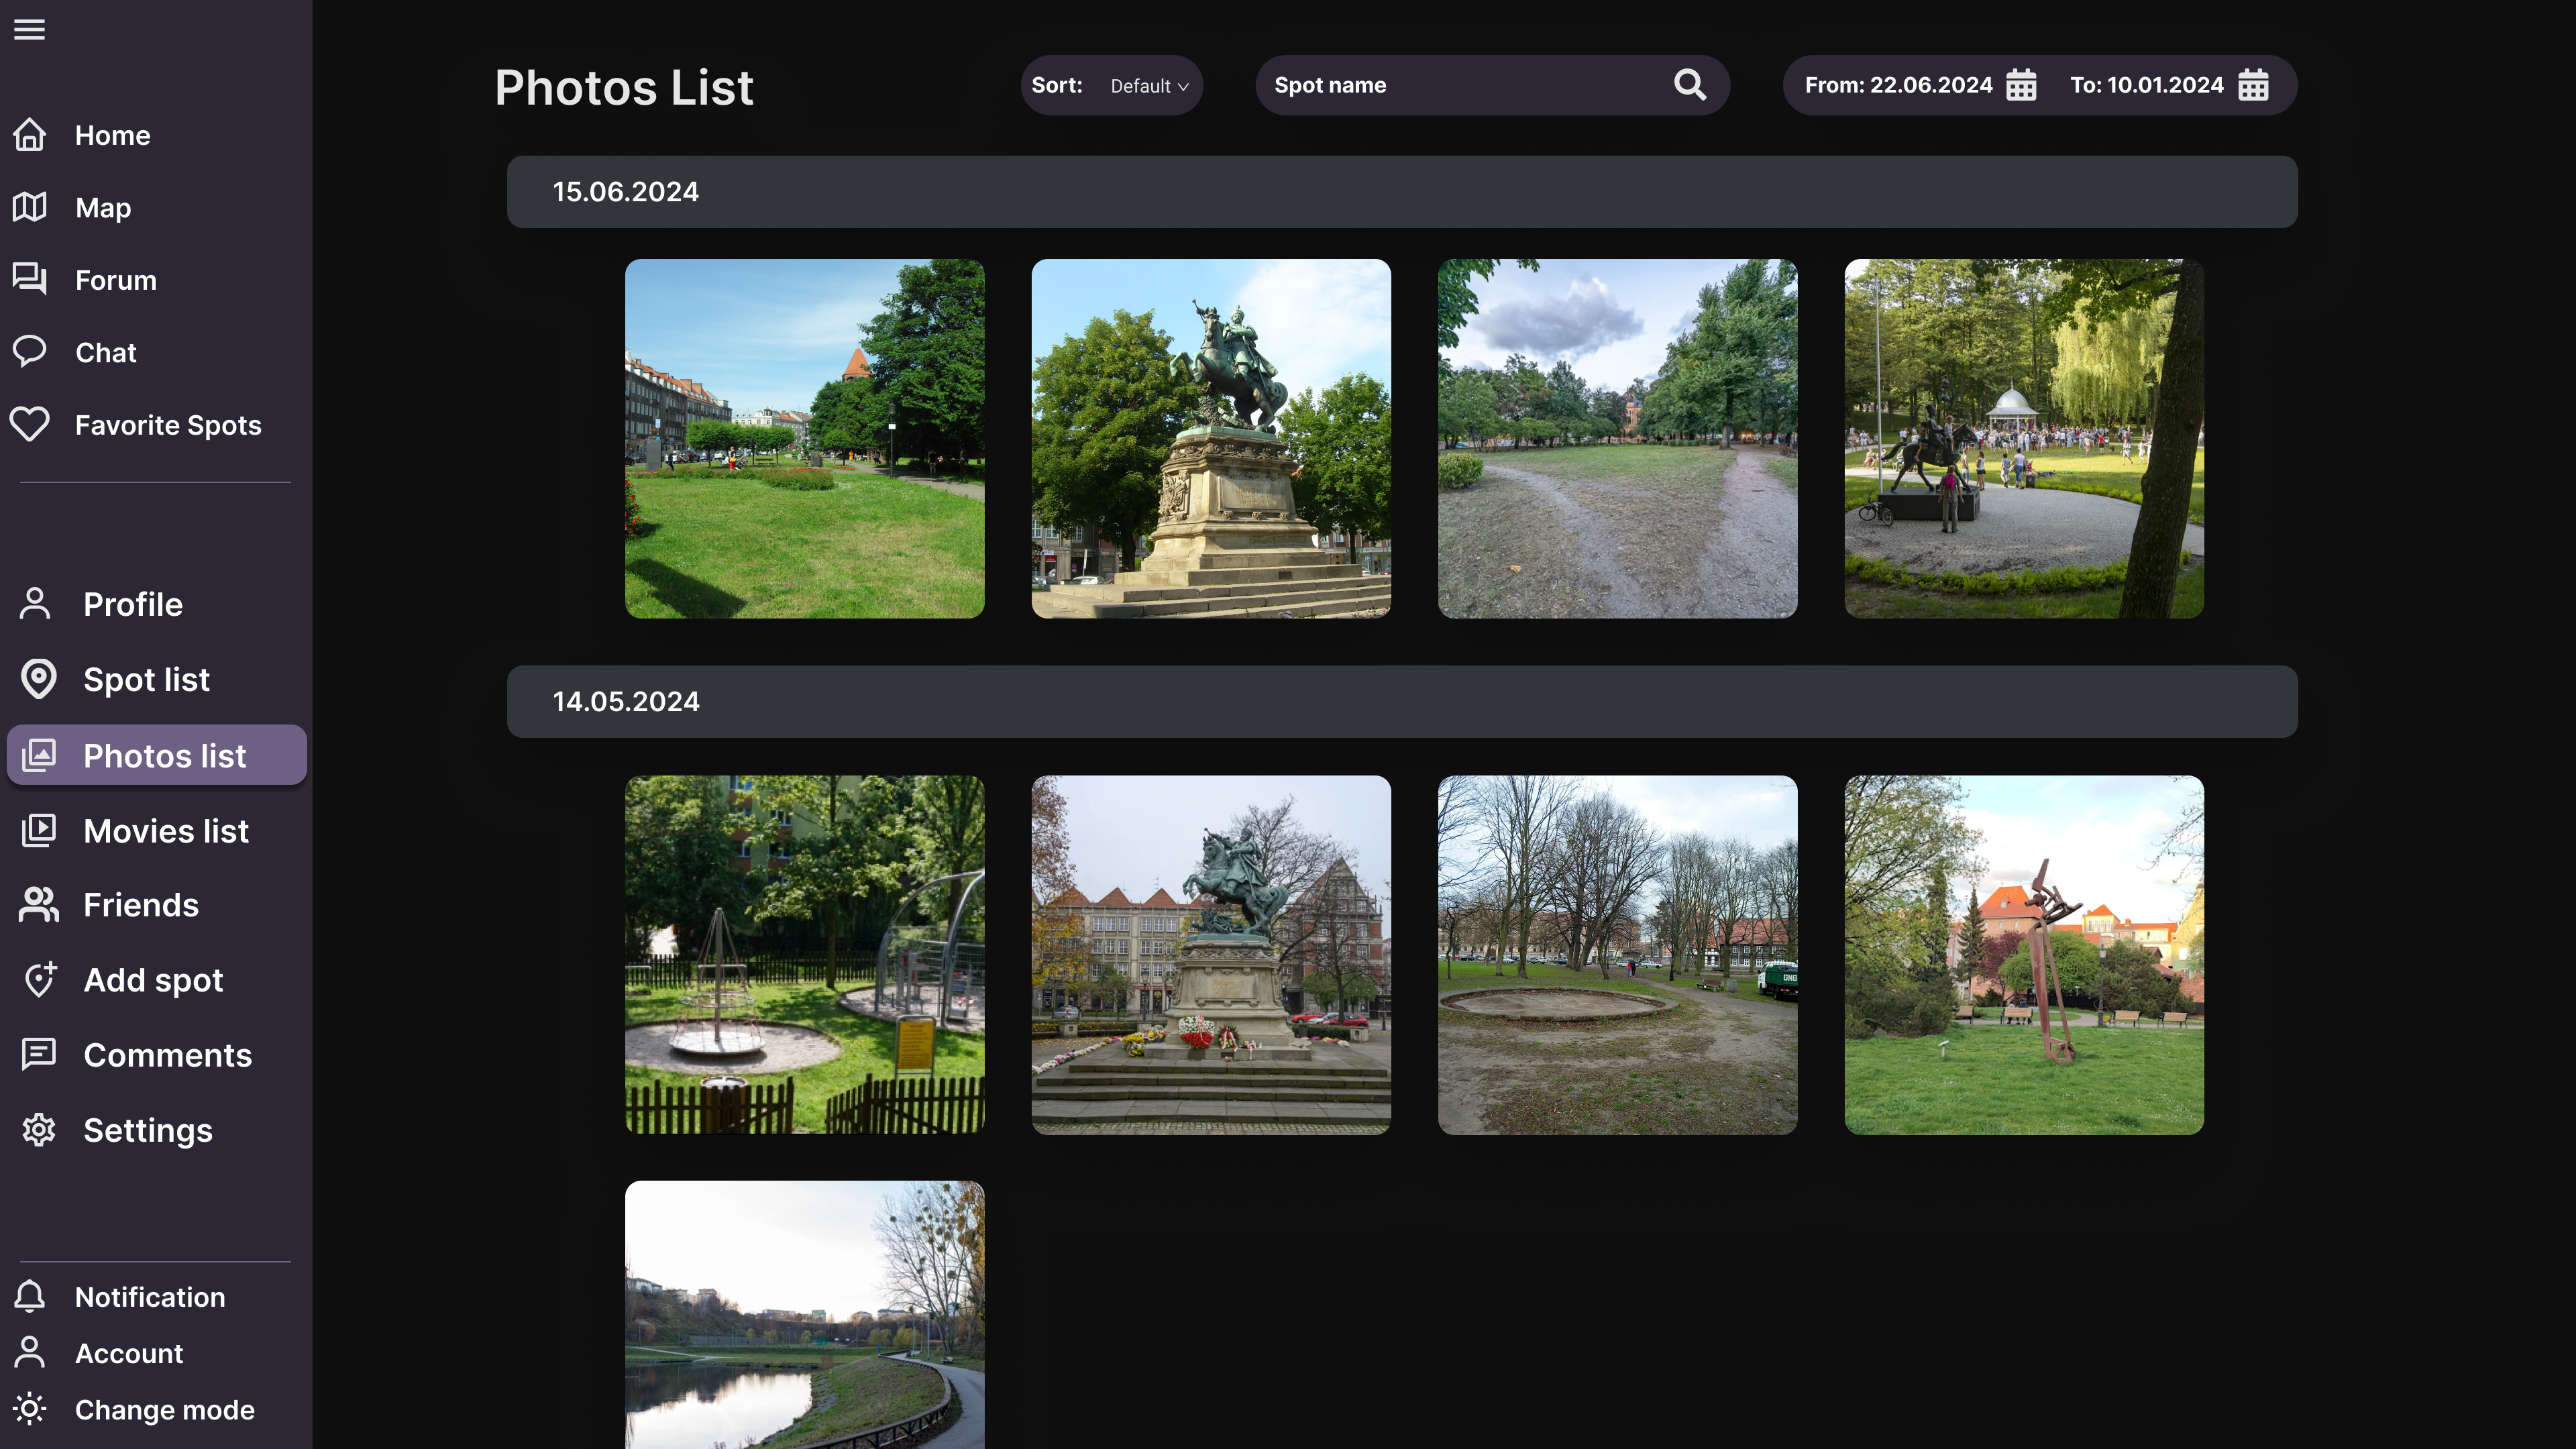
\includegraphics[width=1\textwidth]{attachments/prezentacja-systemu/panel-uzytkownika/photos}
    \caption{Lista zdjęć użytkownika.}
    \label{fig:photos}
\end{figure}

\begin{figure}[H]
    \centering
    \includegraphics[width=1\textwidth]{attachments/prezentacja-systemu/panel-uzytkownika/photos-empty}
    \caption{Komunikat pustego stanu w przypadku braku zdjęć.}
    \label{fig:photos-empty}
\end{figure}

Listę zdjęć można sortować oraz filtrować (rys. \ref{fig:photos-sort}).
Po ustawieniu parametrów lista jest odświeżana automatycznie (rys. \ref{fig:photos-filtered}).

\begin{figure}[H]
    \centering
    \includegraphics[width=1\textwidth]{attachments/prezentacja-systemu/panel-uzytkownika/photos-sort}
    \caption{Opcje sortowania i filtrowania listy zdjęć.}
    \label{fig:photos-sort}
\end{figure}

\begin{figure}[H]
    \centering
    \includegraphics[width=1\textwidth]{attachments/prezentacja-systemu/panel-uzytkownika/photos-filtered}
    \caption{Widok listy zdjęć po zastosowaniu filtrów/sortowania.}
    \label{fig:photos-filtered}
\end{figure}

Po najechaniu na zdjęcie wyświetlany jest przyciemniony pasek ze statystykami (analogicznie jak w profilu),
co pokazano na rys. \ref{fig:photos-hover}.
Dostępny jest również tryb ciemny (rys. \ref{fig:photos-dark}).

\begin{figure}[H]
    \centering
    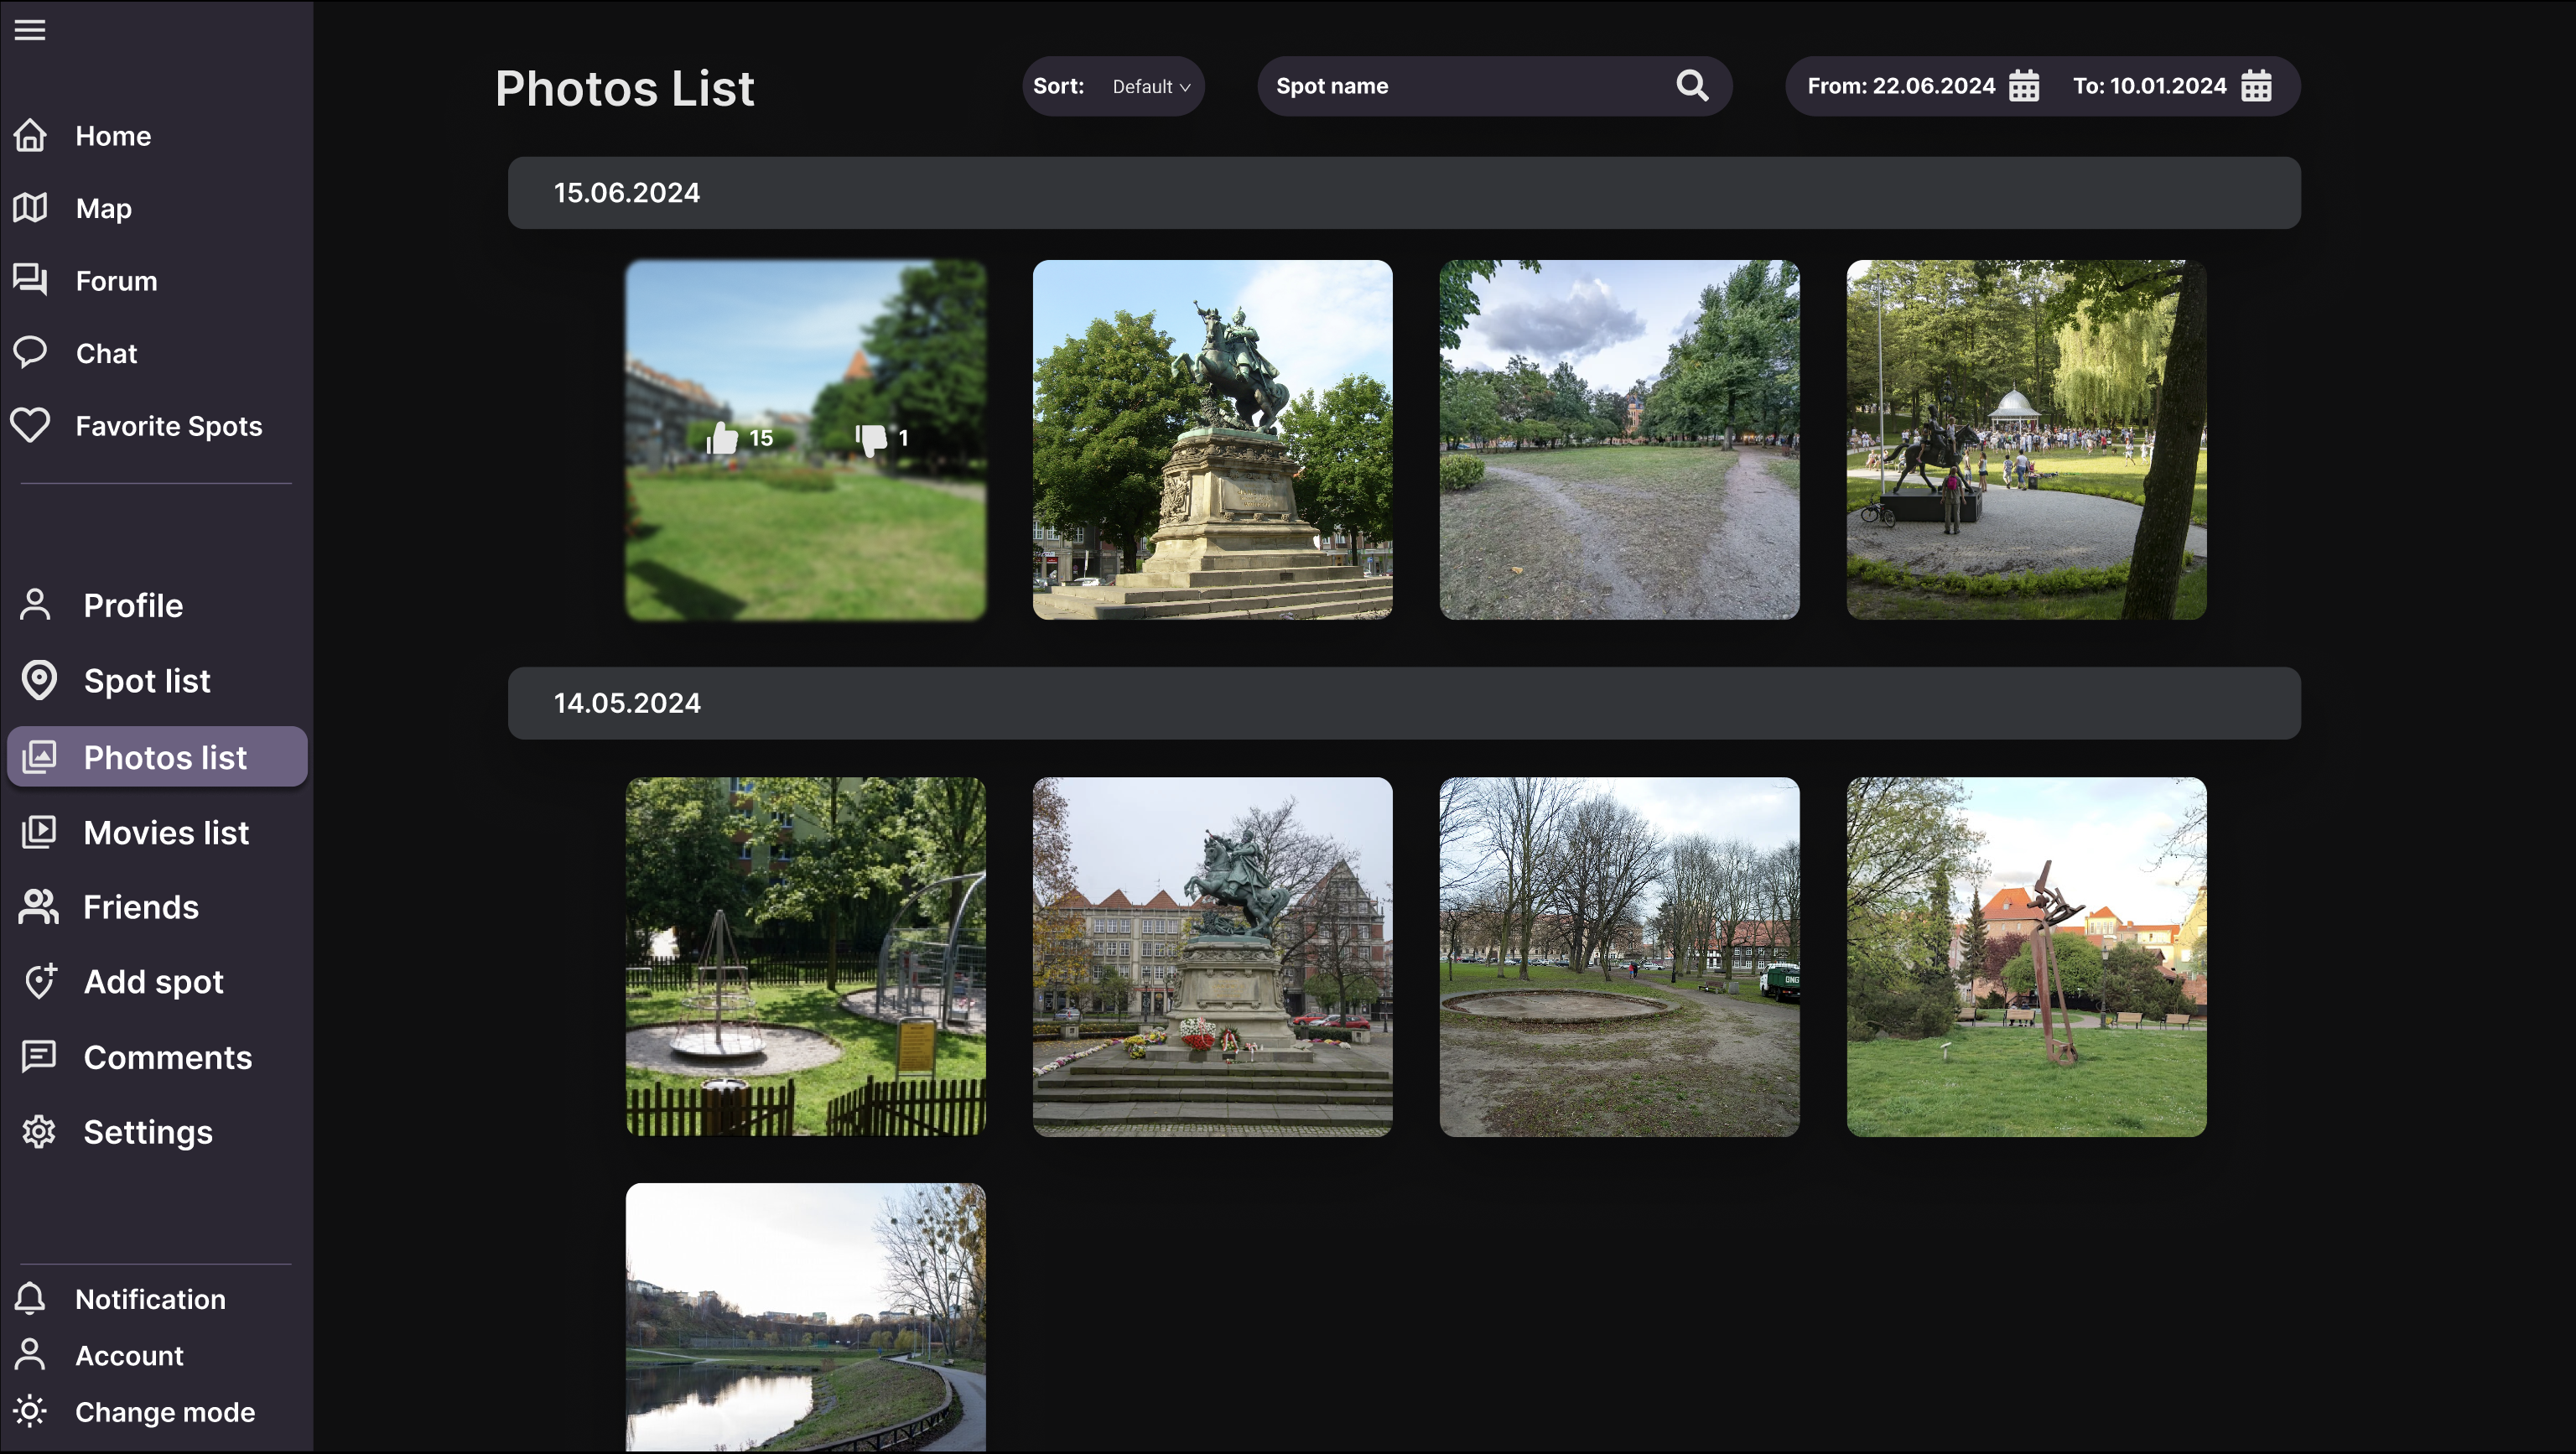
\includegraphics[width=1\textwidth]{attachments/prezentacja-systemu/panel-uzytkownika/photos-hover}
    \caption{Efekt najechania na kafelek zdjęcia (prezentacja statystyk).}
    \label{fig:photos-hover}
\end{figure}

\begin{figure}[H]
    \centering
    \includegraphics[width=1\textwidth]{attachments/prezentacja-systemu/panel-uzytkownika/photos-dark}
    \caption{Lista zdjęć w trybie ciemnym.}
    \label{fig:photos-dark}
\end{figure}

\subsubsection{Movies}

Sekcja \textit{Movies} prezentuje listę filmów dodanych przez użytkownika (rys. \ref{fig:movies}).
W przypadku braku filmów wyświetlany jest komunikat pustego stanu (rys. \ref{fig:movies-empty}).
Dostępne są analogiczne mechanizmy filtrowania i sortowania jak w sekcji \textit{Photos}.

\begin{figure}[H]
    \centering
    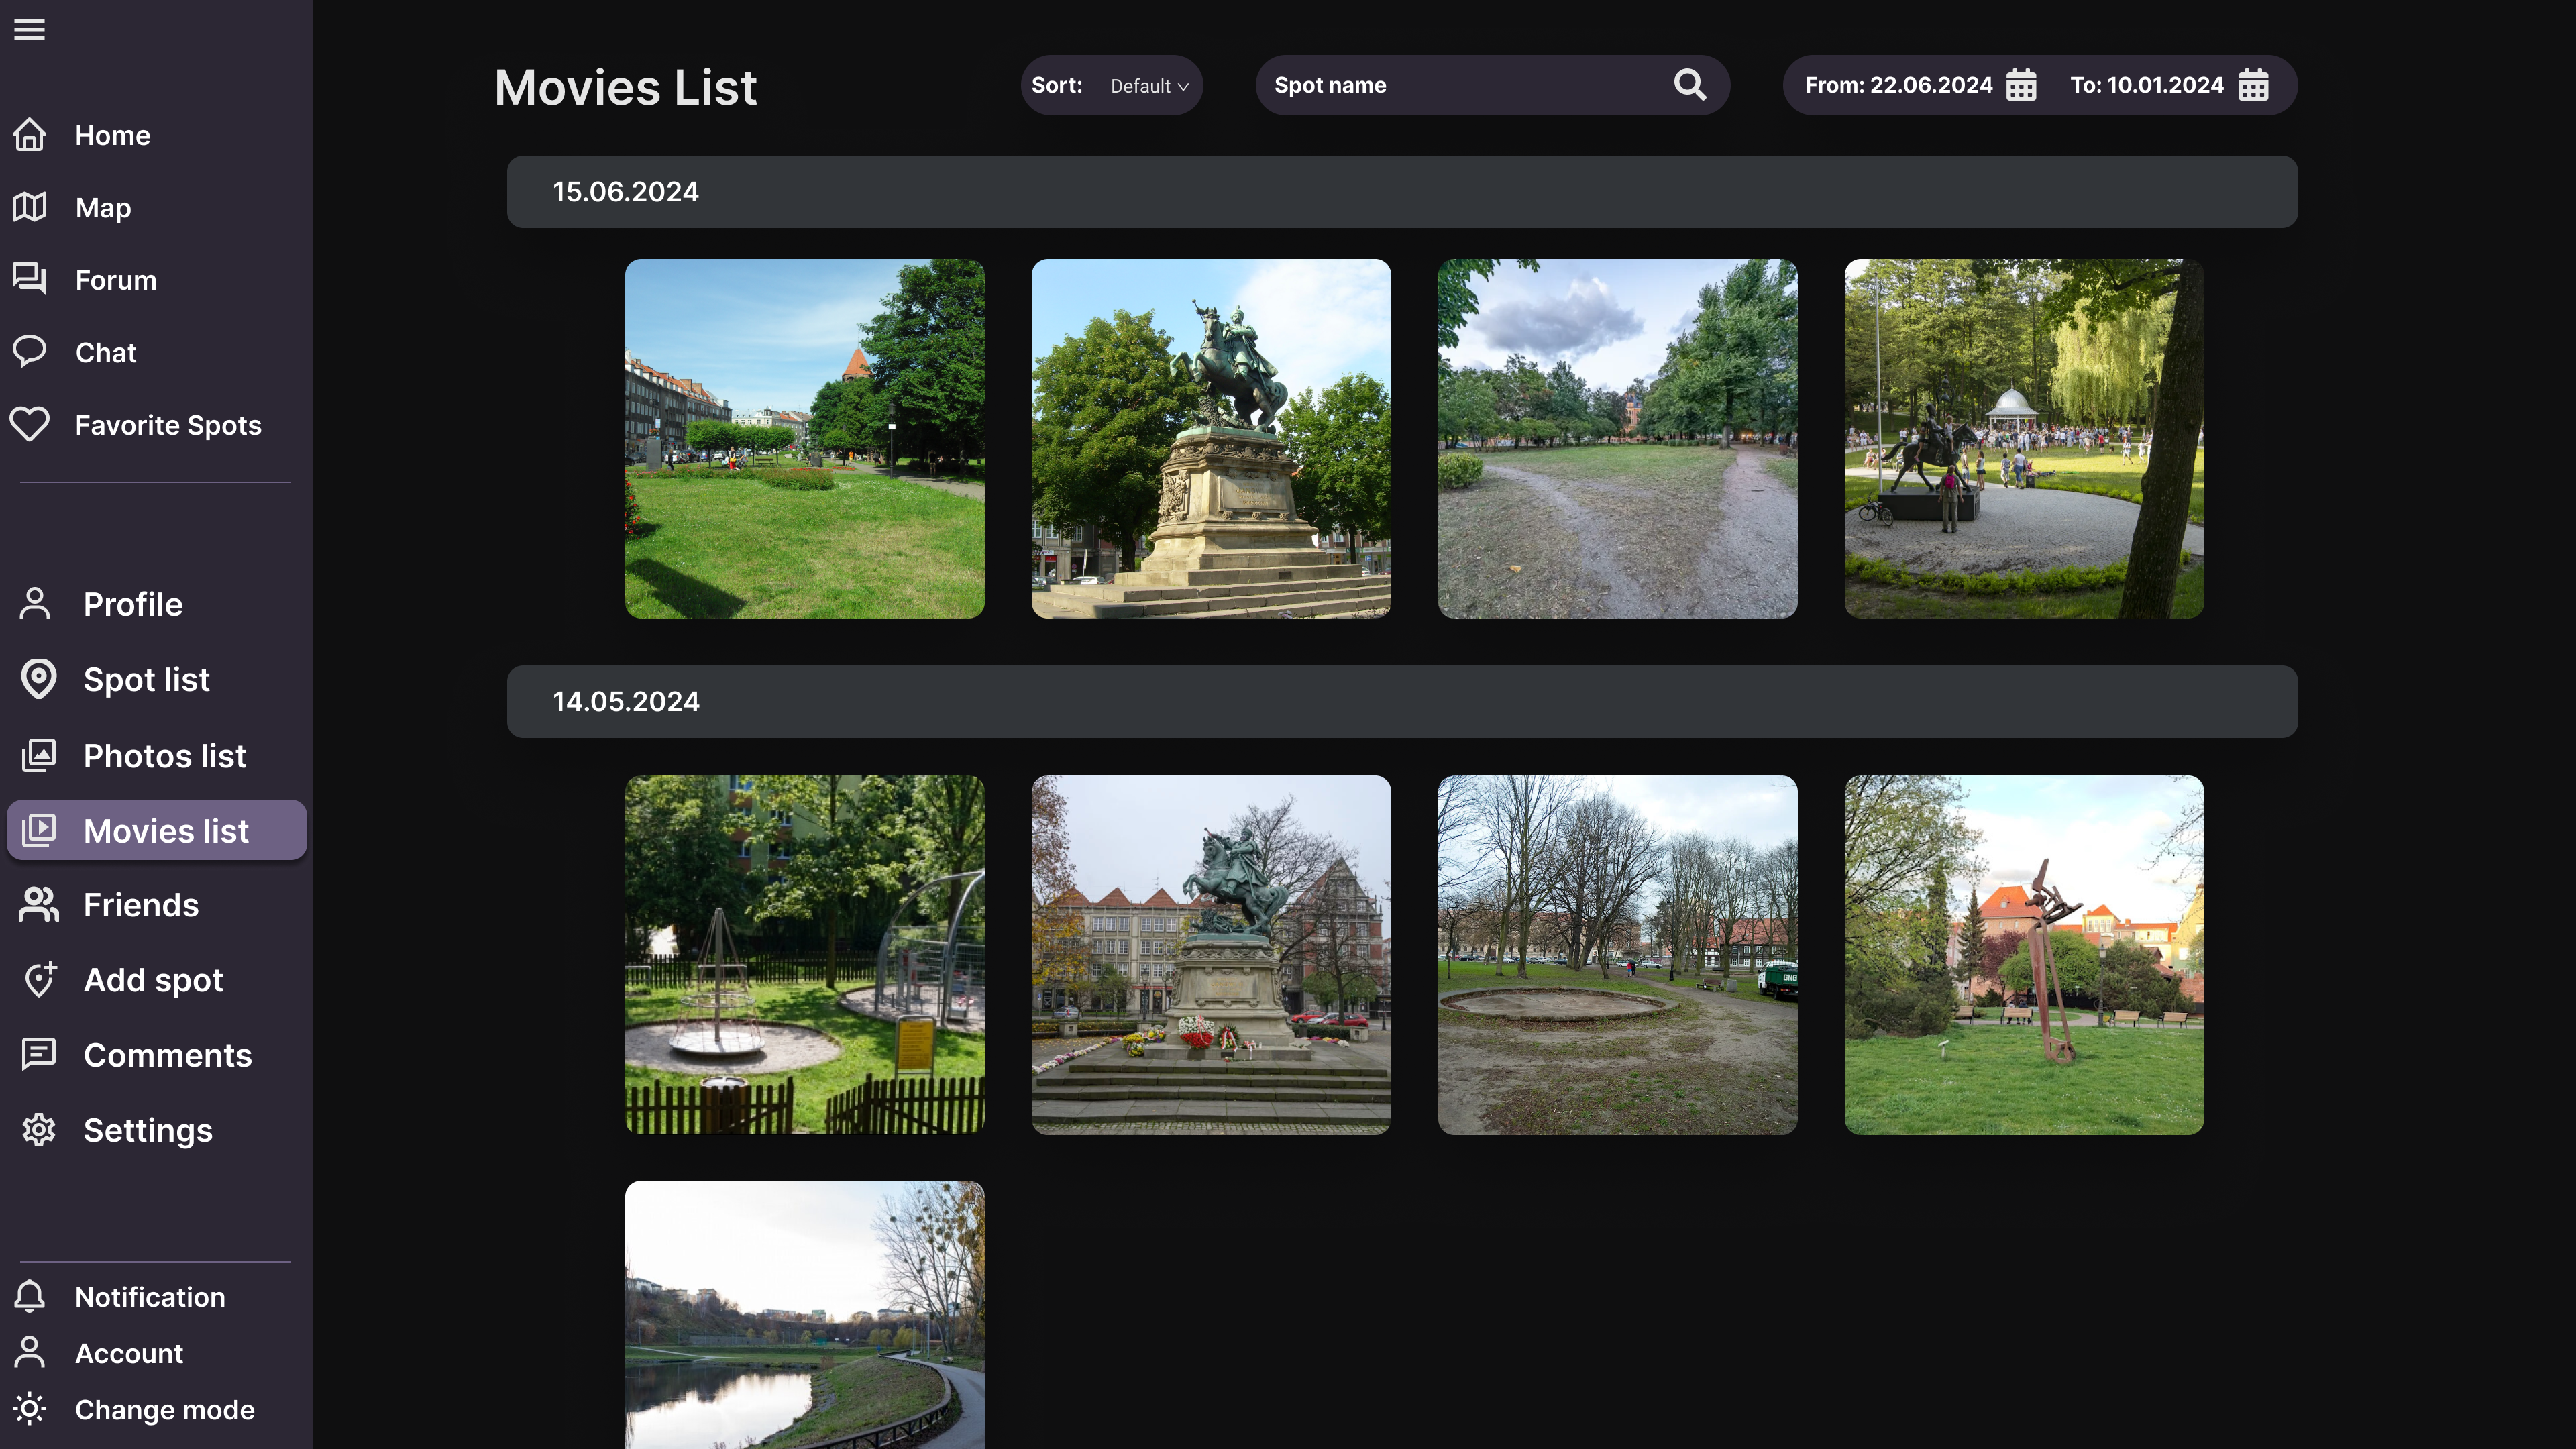
\includegraphics[width=1\textwidth]{attachments/prezentacja-systemu/panel-uzytkownika/movies}
    \caption{Lista filmów użytkownika.}
    \label{fig:movies}
\end{figure}

\begin{figure}[H]
    \centering
    \includegraphics[width=1\textwidth]{attachments/prezentacja-systemu/panel-uzytkownika/movies-empty}
    \caption{Komunikat pustego stanu w przypadku braku filmów.}
    \label{fig:movies-empty}
\end{figure}

Po najechaniu na kafelek filmu prezentowane są statystyki w przyciemnionym polu (rys. \ref{fig:movies-hover}).
Widok w trybie ciemnym pokazano na rys. \ref{fig:movies-dark}.

\begin{figure}[H]
    \centering
    \includegraphics[width=1\textwidth]{attachments/prezentacja-systemu/panel-uzytkownika/movies-hover}
    \caption{Efekt najechania na film (prezentacja statystyk).}
    \label{fig:movies-hover}
\end{figure}

\begin{figure}[H]
    \centering
    \includegraphics[width=1\textwidth]{attachments/prezentacja-systemu/panel-uzytkownika/movies-dark}
    \caption{Lista filmów w trybie ciemnym.}
    \label{fig:movies-dark}
\end{figure}

\subsubsection{Social}

Sekcja \textit{Social} udostępnia trzy listy: znajomych, obserwowanych oraz obserwujących
(rys. \ref{fig:social-friends}--\ref{fig:social-followers}).
Każdy kafelek użytkownika zawiera przyciski akcji (przejście do profilu, rozpoczęcie rozmowy, usunięcie).

\begin{figure}[H]
    \centering
    \includegraphics[width=1\textwidth]{attachments/prezentacja-systemu/panel-uzytkownika/social-friends}
    \caption{Zakładka \textit{Friends} w sekcji Social.}
    \label{fig:social-friends}
\end{figure}

\begin{figure}[H]
    \centering
    \includegraphics[width=1\textwidth]{attachments/prezentacja-systemu/panel-uzytkownika/social-followed}
    \caption{Zakładka \textit{Followed} w sekcji Social.}
    \label{fig:social-followed}
\end{figure}

\begin{figure}[H]
    \centering
    \includegraphics[width=1\textwidth]{attachments/prezentacja-systemu/panel-uzytkownika/social-followers}
    \caption{Zakładka \textit{Followers} w sekcji Social.}
    \label{fig:social-followers}
\end{figure}

Usunięcie znajomego wymaga potwierdzenia w oknie dialogowym (rys. \ref{fig:social-remove}).
Po zaakceptowaniu akcja jest wykonywana, a lista odświeżana (rys. \ref{fig:social-removed}).

\begin{figure}[H]
    \centering
    \includegraphics[width=1\textwidth]{attachments/prezentacja-systemu/panel-uzytkownika/social-remove}
    \caption{Okno potwierdzenia usunięcia użytkownika ze znajomych.}
    \label{fig:social-remove}
\end{figure}

\begin{figure}[H]
    \centering
    \includegraphics[width=1\textwidth]{attachments/prezentacja-systemu/panel-uzytkownika/social-removed}
    \caption{Lista znajomych po usunięciu wybranego użytkownika.}
    \label{fig:social-removed}
\end{figure}

Dodawanie nowych znajomych realizowane jest przez okno modalne z polem wyszukiwania po nazwie użytkownika
(rys.~\ref{fig:social-search}).
W trakcie wpisywania wyświetlana jest lista pasujących wyników (rys.~\ref{fig:social-search2}).
Po wysłaniu zaproszenia adresat widzi je w oknie zaproszeń dostępnym po kliknięciu przycisku
\textit{See friend invites} (rys.~\ref{fig:social-invites}).
Jeśli brak zaproszeń, prezentowany jest komunikat pustego stanu (rys.~\ref{fig:social-invites-empty}).

\begin{figure}[H]
    \centering
    \includegraphics[width=1\textwidth]{attachments/prezentacja-systemu/panel-uzytkownika/social-search}
    \caption{Okno wyszukiwania użytkownika podczas dodawania znajomego.}
    \label{fig:social-search}
\end{figure}

\begin{figure}[H]
    \centering
    \includegraphics[width=1\textwidth]{attachments/prezentacja-systemu/panel-uzytkownika/social-search2}
    \caption{Wyniki wyszukiwania użytkowników podczas dodawania znajomego.}
    \label{fig:social-search2}
\end{figure}

\begin{figure}[H]
    \centering
    \includegraphics[width=1\textwidth]{attachments/prezentacja-systemu/panel-uzytkownika/social-invites}
    \caption{Okno zaproszeń do znajomych z możliwością akceptacji/odrzucenia.}
    \label{fig:social-invites}
\end{figure}

\begin{figure}[H]
    \centering
    \includegraphics[width=1\textwidth]{attachments/prezentacja-systemu/panel-uzytkownika/social-invites-empty}
    \caption{Komunikat pustego stanu dla okna zaproszeń (brak zaproszeń).}
    \label{fig:social-invites-empty}
\end{figure}

W sekcji dostępny jest także tryb ciemny (rys.~\ref{fig:social-dark}).

\begin{figure}[H]
    \centering
    \includegraphics[width=1\textwidth]{attachments/prezentacja-systemu/panel-uzytkownika/social-dark}
    \caption{Sekcja Social w trybie ciemnym.}
    \label{fig:social-dark}
\end{figure}

\subsubsection{Add spot}

Sekcja \textit{Add spot} prezentuje listę \glslink{spot}{spotów} dodanych przez użytkownika do aplikacji (rys.~\ref{fig:add-spot-full}).
W przypadku braku wpisów wyświetlany jest komunikat pustego stanu (rys.~\ref{fig:add-spot-empty}).
W prawym górnym rogu dostępny jest przycisk \textit{Add Spot}, który otwiera formularz dodawania
nowego \glslink{spot}{spota} (rys.~\ref{fig:add-spot-form}).

\begin{figure}[H]
    \centering
    \includegraphics[width=1\textwidth]{attachments/prezentacja-systemu/panel-uzytkownika/add-spot-full}
    \caption{Lista spotów dodanych przez użytkownika do aplikacji.}
    \label{fig:add-spot-full}
\end{figure}

\begin{figure}[H]
    \centering
    \includegraphics[width=1\textwidth]{attachments/prezentacja-systemu/panel-uzytkownika/add-spot}
    \caption{Komunikat pustego stanu w sekcji Add spot (brak dodanych spotów).}
    \label{fig:add-spot-empty}
\end{figure}

\begin{figure}[H]
    \centering
    \includegraphics[width=1\textwidth]{attachments/prezentacja-systemu/panel-uzytkownika/add-spot-form}
    \caption{Formularz dodawania nowego spota.}
    \label{fig:add-spot-form}
\end{figure}

W formularzu zastosowano walidację danych.
W przypadku braku wymaganych informacji wyświetlane są komunikaty walidacyjne (rys.~\ref{fig:add-spot-error}).

\begin{figure}[H]
    \centering
    \includegraphics[width=1\textwidth]{attachments/prezentacja-systemu/panel-uzytkownika/add-spot-error}
    \caption{Walidacja formularza dodawania spota (komunikaty błędów).}
    \label{fig:add-spot-error}
\end{figure}

Dla załączonych miniatur zdjęć przewidziano interakcję usuwania: po najechaniu pojawia się przyciemnienie,
a kliknięcie powoduje usunięcie miniatury (rys.~\ref{fig:add-spot-hover}).
Widok w trybie ciemnym przedstawiono na rys.~\ref{fig:add-spot-dark}.

\begin{figure}[H]
    \centering
    \includegraphics[width=1\textwidth]{attachments/prezentacja-systemu/panel-uzytkownika/add-spot-hover}
    \caption{Interakcja usunięcia miniatury zdjęcia w formularzu (hover).}
    \label{fig:add-spot-hover}
\end{figure}

\begin{figure}[H]
    \centering
    \includegraphics[width=1\textwidth]{attachments/prezentacja-systemu/panel-uzytkownika/add-spot-dark}
    \caption{Sekcja Add spot w trybie ciemnym.}
    \label{fig:add-spot-dark}
\end{figure}

\subsubsection{Comments}

Sekcja \textit{Comments} prezentuje listę komentarzy dodanych przez użytkownika (rys.~\ref{fig:comments}).
Układ oraz sposób prezentacji nawiązuje do list zdjęć i filmów.
Jeśli brak komentarzy, wyświetlany jest komunikat pustego stanu (rys.~\ref{fig:comments-empty}).
Dostępny jest także tryb ciemny (rys.~\ref{fig:comments-dark}).

\begin{figure}[H]
    \centering
    \includegraphics[width=1\textwidth]{attachments/prezentacja-systemu/panel-uzytkownika/comments}
    \caption{Lista komentarzy użytkownika.}
    \label{fig:comments}
\end{figure}

\begin{figure}[H]
    \centering
    \includegraphics[width=1\textwidth]{attachments/prezentacja-systemu/panel-uzytkownika/comments-empty}
    \caption{Komunikat pustego stanu w sekcji Comments (brak komentarzy).}
    \label{fig:comments-empty}
\end{figure}

\begin{figure}[H]
    \centering
    \includegraphics[width=1\textwidth]{attachments/prezentacja-systemu/panel-uzytkownika/comments-dark}
    \caption{Sekcja Comments w trybie ciemnym.}
    \label{fig:comments-dark}
\end{figure}

\subsubsection{Settings}

Ostatnią sekcją są ustawienia konta.
Prezentowane są podstawowe dane (nazwa użytkownika, e-mail, hasło) wraz z przyciskami \textit{Edit} (rys.~\ref{fig:settings}).
Po wybraniu edycji w prawym obszarze widoku pojawia się odpowiedni formularz zmiany danych: nazwy
użytkownika (rys.~\ref{fig:settings-username}), adresu e-mail (rys.~\ref{fig:settings-email}) lub
hasła (rys.~\ref{fig:settings-password}). W przypadku hasła przewidziano pola na stare hasło,
nowe hasło oraz potwierdzenie.

\begin{figure}[H]
    \centering
    \includegraphics[width=1\textwidth]{attachments/prezentacja-systemu/panel-uzytkownika/settings}
    \caption{Widok ustawień konta (Account details).}
    \label{fig:settings}
\end{figure}

\begin{figure}[H]
    \centering
    \includegraphics[width=1\textwidth]{attachments/prezentacja-systemu/panel-uzytkownika/settings-username}
    \caption{Formularz zmiany nazwy użytkownika.}
    \label{fig:settings-username}
\end{figure}

\begin{figure}[H]
    \centering
    \includegraphics[width=1\textwidth]{attachments/prezentacja-systemu/panel-uzytkownika/settings-email}
    \caption{Formularz zmiany adresu e-mail.}
    \label{fig:settings-email}
\end{figure}

\begin{figure}[H]
    \centering
    \includegraphics[width=1\textwidth]{attachments/prezentacja-systemu/panel-uzytkownika/settings-password}
    \caption{Formularz zmiany hasła (stare hasło, nowe hasło, potwierdzenie).}
    \label{fig:settings-password}
\end{figure}

Dla ustawień przygotowano również wariant ciemny (rys.~\ref{fig:settings-dark}), w którym dostosowano kontrast
pól formularzy i elementów nawigacji.

\begin{figure}[H]
    \centering
    \includegraphics[width=1\textwidth]{attachments/prezentacja-systemu/panel-uzytkownika/settings-dark}
    \caption{Ustawienia konta w trybie ciemnym.}
    \label{fig:settings-dark}
\end{figure}

